{\let\clearpage\relax
\chapter{Ablauforganisation}}
\label{sec:ablauforganisation}

\section{Einsatz des Spiralmodells}
Im Projekt zur Entwicklung eines Datenaufbereitungssystems für ein Krankenhaus kommt das Spiralmodell zum Einsatz, um iterative Entwicklung und systematisches Risikomanagement miteinander zu verbinden. Aufgrund der langen Laufzeit, der hohen Komplexität sowie ethischer und datenschutzrechtlicher Anforderungen eignet sich dieses Vorgehensmodell besonders.

\begin{figure}[ht]
  \centering
  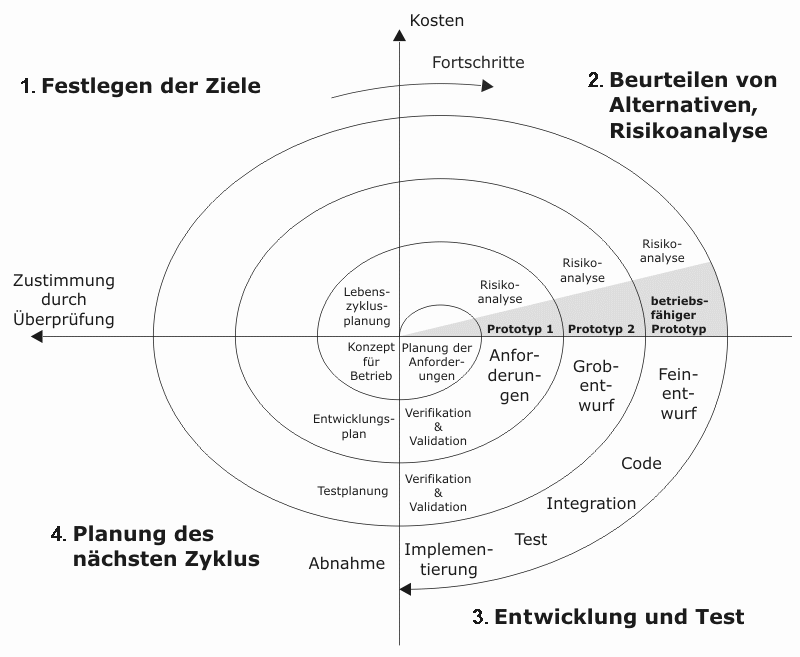
\includegraphics[width=0.6\textwidth]{fig/Spiralmodel_nach_Boehm.png}
  \caption{Das Spiralmodell im Projektkontext}
\end{figure}

\section{Umsetzung Teams und Kommunikation}
Die Umsetzung erfolgt durch zwei parallel arbeitende Teams: eines für die Benutzeroberfläche (UI) und eines für die Datenverarbeitung (Data). Beide Teams arbeiten eigenständig in jeweils eigenen Spiralzyklen. Die Kommunikation erfolgt über definierte Schnittstellen und wird durch die Teamleiter koordiniert. Fachliche Fragen stimmen die Teams bei Bedarf mit IT, ärztlichem Personal, Klinikleitung und Datenschutzbeauftragten ab. Die Infrastrukturverantwortung liegt beim Data-Team, juristische Fragestellungen werden durch interne oder externe Juristen begleitet.

% Bildvorschlag: Kommunikationsstruktur aus Folie 6 oder 7
\begin{figure}[ht]
  \centering
  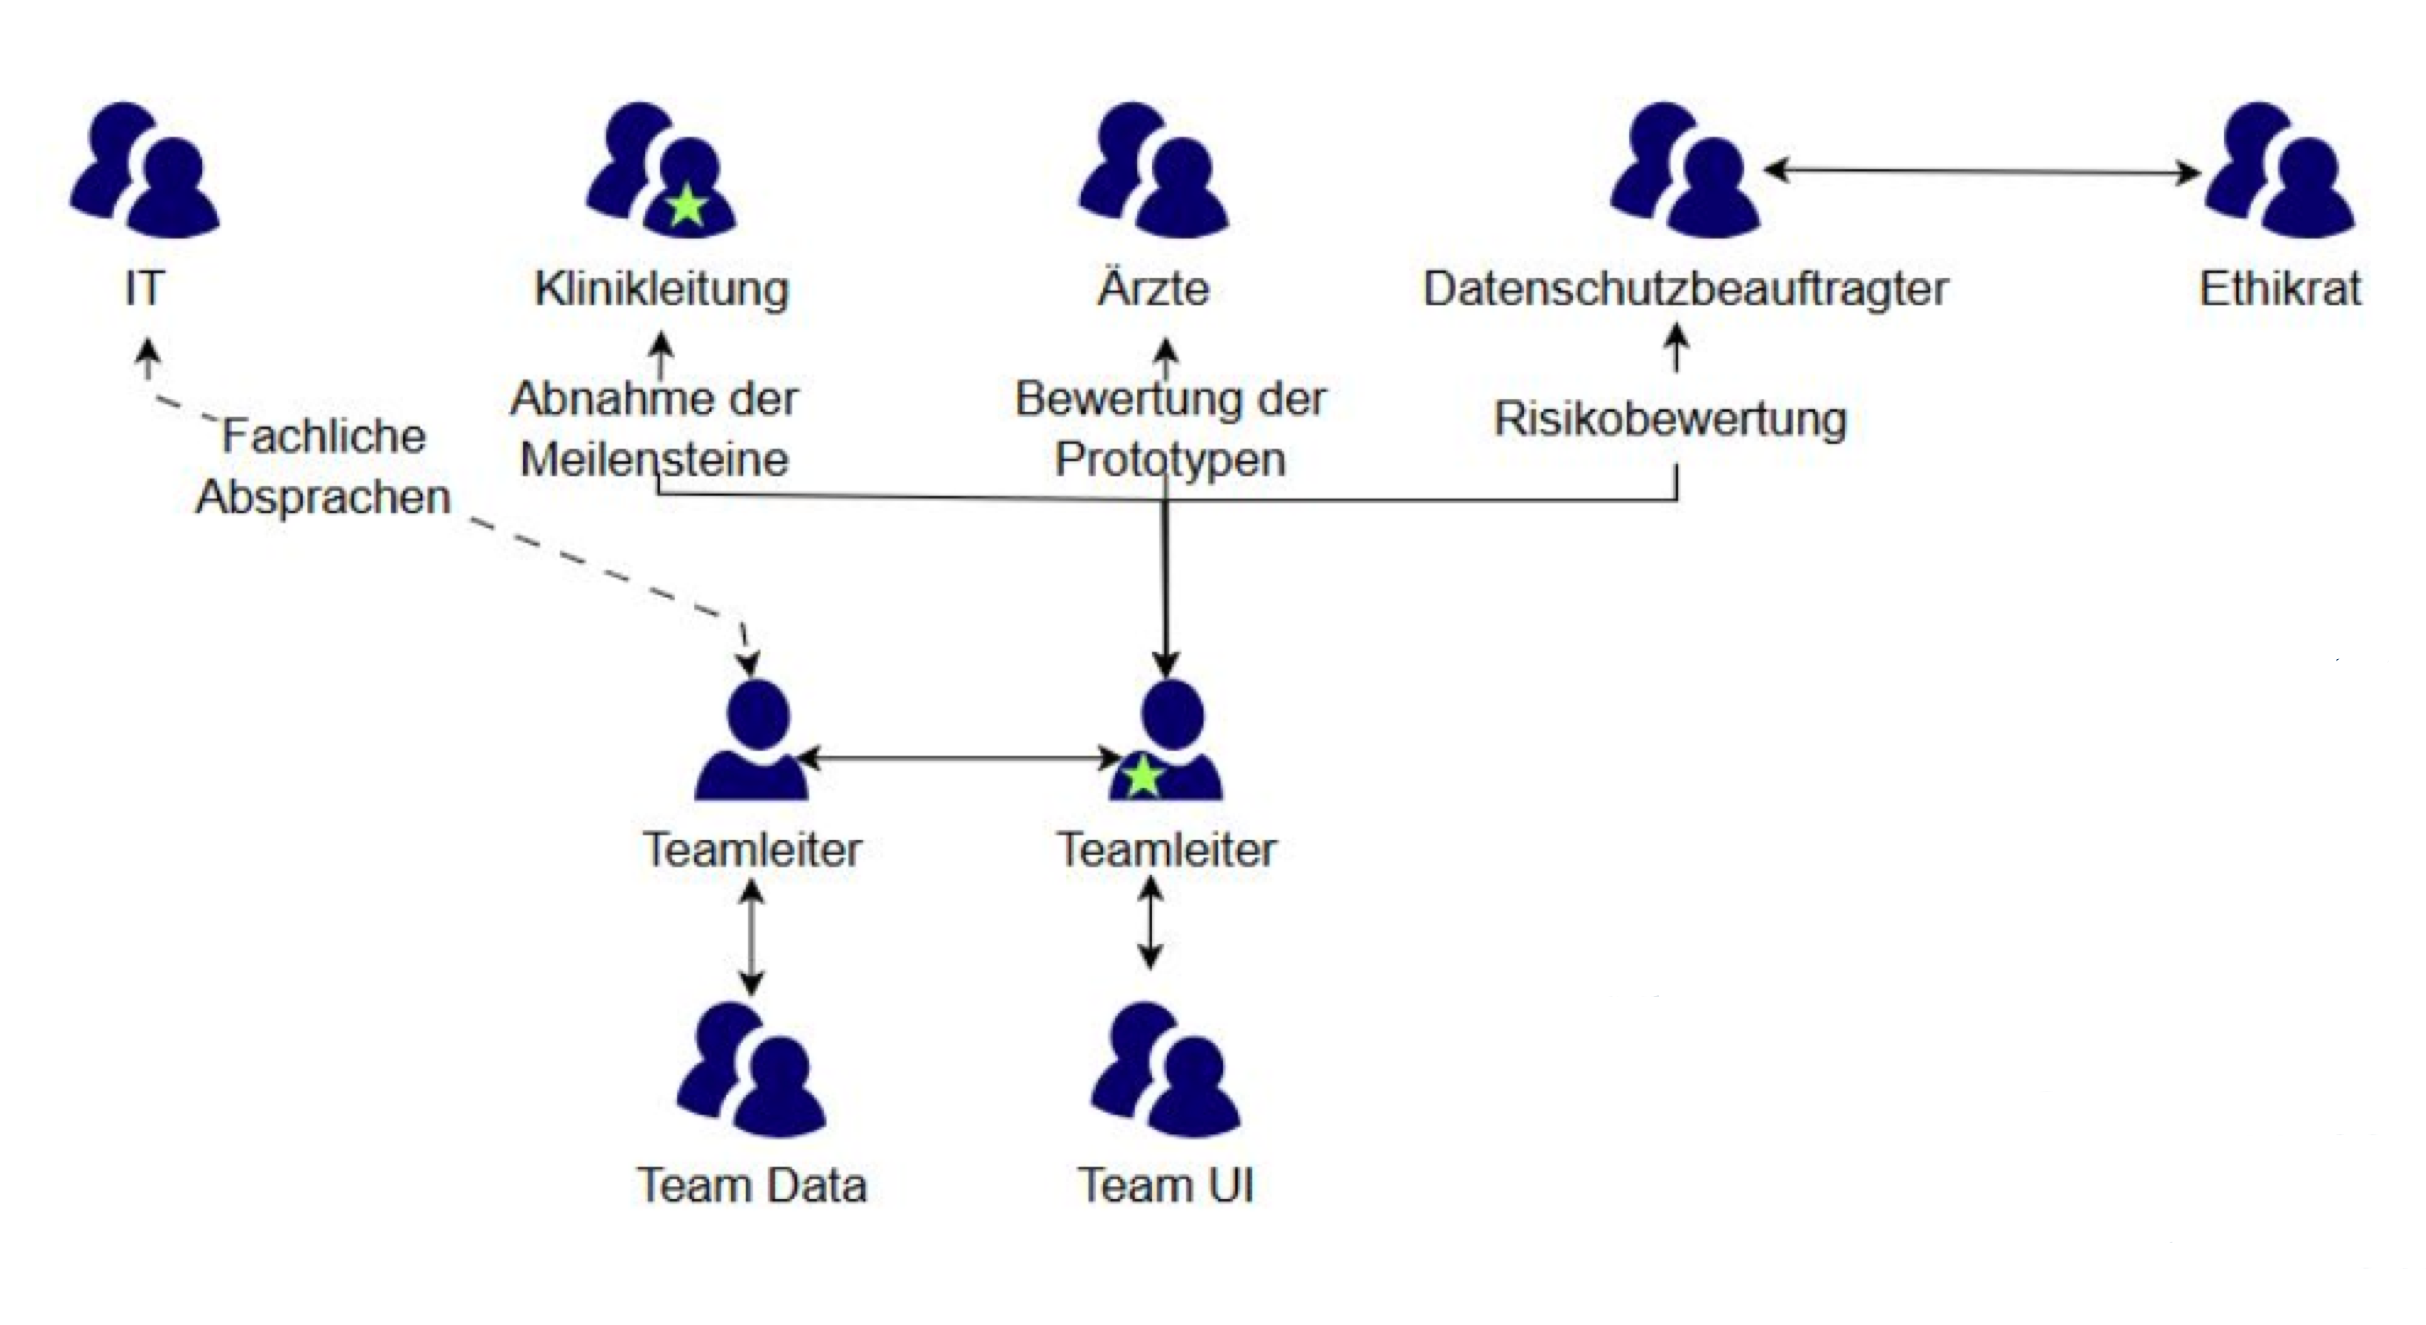
\includegraphics[width=0.8\textwidth]{fig/kommunikation.png}
  \caption{Kommunikationsstruktur der Projektteams}
\end{figure}

\section{Spiralzyklen}
Der Ablauf gliedert sich in mehrere Spiralzyklen mit jeweils definierten Zielen, Risikoanalysen, Entwicklungsmaßnahmen und Evaluationen:

\textbf{Durchlauf 0 – Projektplanung:} In dieser Phase erfolgt die Bedarfsanalyse, die Zieldefinition, eine Technologie-Evaluation sowie die Kosten- und Zeitplanung. Die Projektstruktur wird festgelegt, Interviews mit relevanten Stakeholdern werden geführt und die juristische Prüfung schließt den Durchlauf ab.

% Bildvorschlag: Ablaufplan aus Folie 8
\begin{figure}[ht]
  \centering
  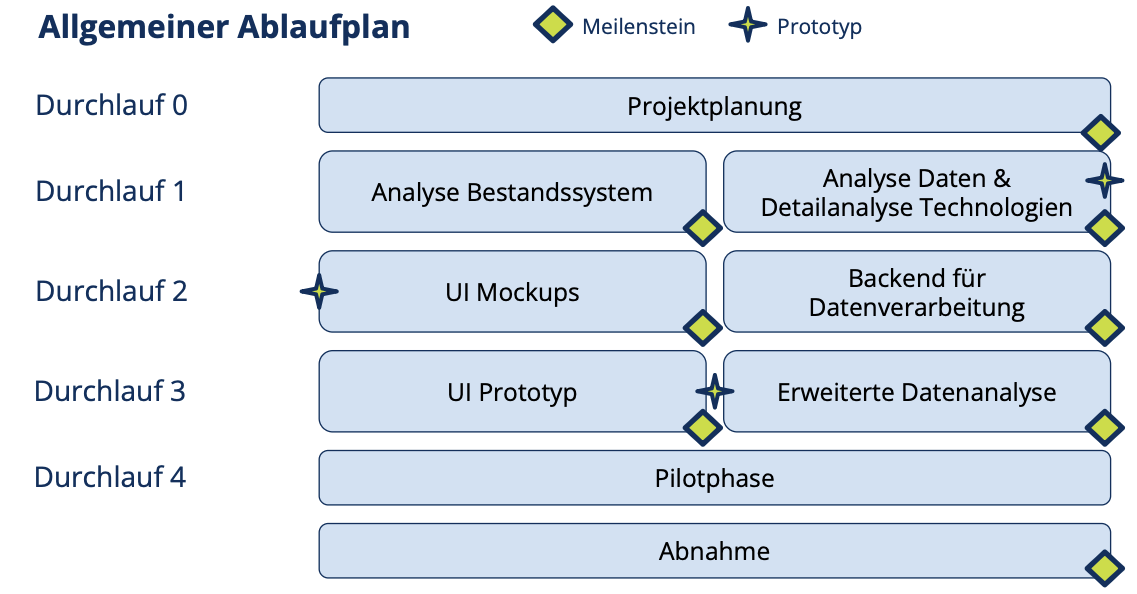
\includegraphics[width=\textwidth]{fig/ablaufplan.png}
  \caption{Übersicht über die Spiralzyklen}
\end{figure}

\textbf{Durchlauf 1 – Analyse des Bestandssystems:} Das UI-Team analysiert reale Nutzungsszenarien und dokumentiert typische Workflows gemeinsam mit medizinischem Personal. Gleichzeitig bewertet das Data-Team verfügbare Technologien hinsichtlich Datenschutz, Kompatibilität und Funktionalität.

\textbf{Durchlauf 2 – Mockup und Backend:} Das UI-Team erstellt klickbare Mockups auf Basis synthetischer Daten und bewertet sie anhand von Effizienzkriterien wie Klickanzahl und Nutzerfeedback. Das Data-Team entwickelt erste Scraper sowie ein zentrales Backend zur normgerechten Aggregation und Speicherung der Daten.

\textbf{Durchlauf 3 – Funktionale Prototypen:} Das UI-Team entwickelt ein interaktives Dashboard mit rollenbasiertem Zugriff, mobiler Unterstützung, Barrierefreiheit und KI-gestützter Datenverarbeitung. Funktionen wie ein „ChatGPT“-ähnliches Interface und eine Anomalieerkennung kommen zum Einsatz. Parallel entwickelt das Data-Team ein Language Model zur erweiterten Analyse und Korrelation der Daten.

\textbf{Durchlauf 4 – Pilotphase und Abnahme:} Das Gesamtsystem wird in einer Pilotumgebung konfiguriert und unter Echtbedingungen getestet. Monitoring, Nutzerschulung und eine normenkonforme Prüfung durch IT, ärztliches Personal, Projektleitung und Datenschutzbeauftragte bilden die Grundlage für die finale Abnahme.


Während aller Spiralzyklen erfolgt eine kontinuierliche Risikobewertung. Besondere Aufmerksamkeit gilt dabei der Datensicherheit, der Integration von KI-Komponenten sowie der Systemkompatibilität. Der Ethikrat ist stets eingebunden, sobald nicht-synthetische Daten oder automatisierte Entscheidungsprozesse ins Spiel kommen. Für KI-Komponenten werden ISO/IEC-Normen beachtet. Die Evaluation des UI basiert unter anderem auf Nutzerfeedback über Systeme wie den SUS oder den UEQ.
